\chapter{Linus Torvalds on Git}

After watching \href{https://www.youtube.com/watch?v=4XpnKHJAok8}{Tech Talk: Linus Torvalds on git} each team member wrote down some notes.

\section{Notes Jeroen}
bitkeeper only commercial software which is distributed (around 14 May 2007).
GIT and mercurial are distributed as well.

GIT is fully distributed, every download and working is it's own branch (~15:15 min).
This is a different model which is far more stable and error proof than one central head.

Kernel acceptance is done by network-of-trust (~27:30 min). That's the way that people pull 
updates from each other, only if they trust them. And some are trusted by Linus so will some 
updates eventually come in the kernel.

GIT is focused on easy merging (~35:10 min). If a developer has made changes and the merge 
on a higher level has to many merge conflicts. A developer with knowledge of the code and 
expertise can execute it as well just as easy. 

Question about central version control system is cheaper and easier for small projects 
(~38 min). GIT reserves network traffic because of local branching. Naming branches in central 
based system causes more overhead than an distributed system.

GIT doesn't track a separate file, but the whole project as one (~44:15 min). Searching a 
specific file it will first find the global environment and search for file. This is a bit 
slower than other systems by the way GIT works.

In GIT it is possible to (~48:35 min) make a backbone GIT project and refer to other GIT 
projects. It is also possible to extract certain files of older branches.

Again some explanation that special attention was spend of the development of merging.
(~50:39 min). The system of branching works only well if merging is going well. If merging 
is an issue than branching is a bad decision.

GIT calculates a diff stat after a merge(~54 min). This gives information about the parts 
that have changed since the last merge.

GIT guarantees that unwanted changes (disk errors or whatever) are tracked and warned 
(~65 min). GIT uses SHA-1 but not in a security application but for keeping signatures of 
files. Applied for trusting data.

The development got hacked at bitkeeper (~59:10 min). When that happens you will pay 
attention to detect changes in codes.

Again a part not about tracking separate files but a overview of the whole(~1:03:17 min).

Code is tracked across files. Again an example of tracking with a greater overview and not 
in file level (~1:08:00 min). GIT can tell which code lines come from a file a couple of 
years ago.

\vspace{2mm}

Source: \href{https://www.os3.nl/2015-2016/students/jeroen_van_prooijen/es/week39#youtube}{Wiki, Jeroen van Prooijen}

\section{Notes Mike}
The video mainly serves as basic introduction to Git, highlighting the thinking process and design goals. During the talk, Torvalds focusses on the following benefits/features:

\begin{itemize}
\item Continue work offline with full functionality
\item Every user has a branch
\item No commit access to a central repository (less politics, more development)
\item Provides concurrent dev/test/release cycles because every team uses it's own repository
\item"Security" relies on network of trust between developers
\item Easy branching/merging of large projects
\end{itemize}

Answers to questions that were asked during the talk were all based on the features above.

\vspace{2mm}

Source: \href{https://www.os3.nl/2015-2016/students/mike_maarse/es/es_ga_wk39_2}{Personal wiki, Mike Maarse}

\chapter{Latex vs. MS Word}

\section{Microsoft Word or LateX?}
\textbf{by Jeroen van Prooijen}\\

\begin{wrapfigure}{r}{0.5\textwidth}
 \vspace{-20pt}
 \begin{center}
  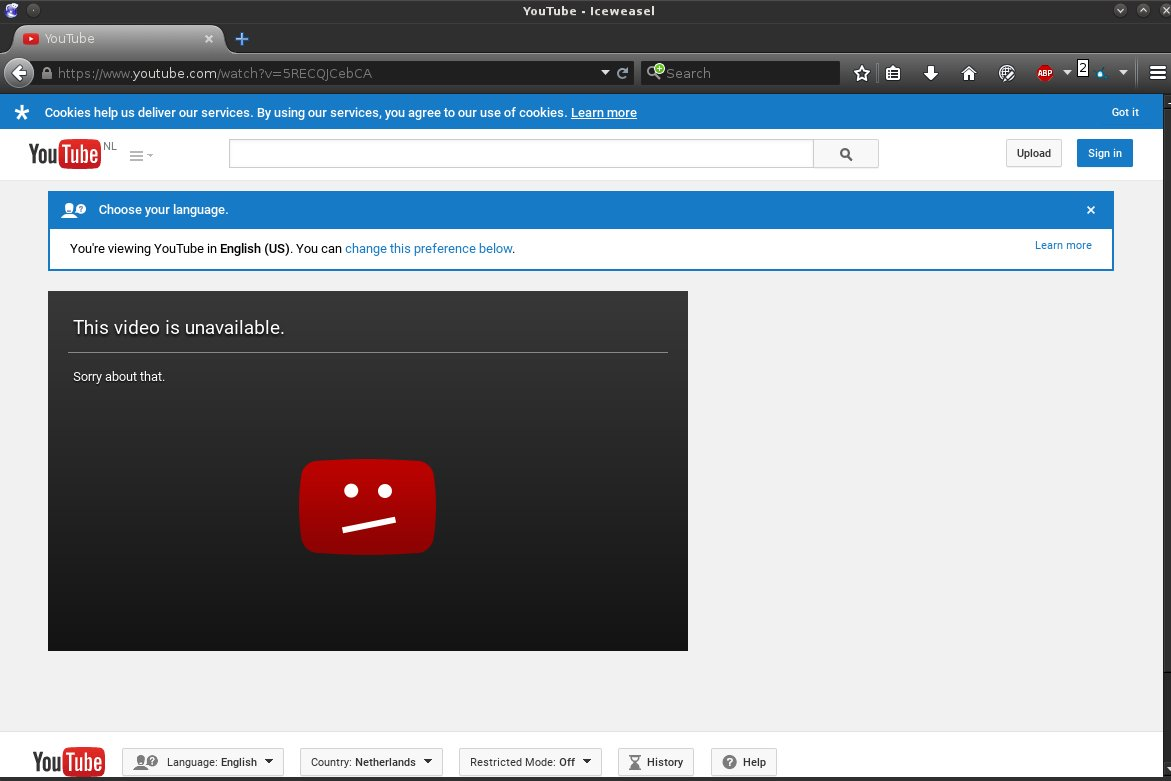
\includegraphics[width=0.5\textwidth]{error_youtube.jpg}
 \end{center}
 \vspace{-20pt}
 \caption{screenshot youtube error}
 \vspace{-10pt}
\label{fig:error_youtube}
\end{wrapfigure}

I tried to watch the following youtube movie: \url{https://www.youtube.com/watch?v=5RECQJCebCA}\\
but it could not be found, see image \ref{fig:error_youtube}. For the placing the image \ref{fig:error_youtube} and wrapping this
text around it I used a explanation on Wikibooks.org\cite{wikibooks_figures}

\section{LaTeX vs Word}
\textbf{by Mike Maarse}\\

This section summarizes the information found on the provided web links to oestrem.com \cite{oestrem} and openwetware.org \cite{openwetware}.

\vspace{2mm}

Personal note: The information on these page date back to 2007 \cite{oestrem} and 2009 \cite{openwetware}. In the meantime both MS Word and Latex have continued development. It would be interesting to see if the comparisons made still hold up...

\subsection{Things Twice - Latex vs. Word vs. Writer}
Although writing \LaTeX documents could be considered "coding", the typesetter offers many benefits over MS Word and LibreOffice Writer. It may look intimidating at first because \LaTeX definitely isn't WYSIWYG. It is when rendering pages that the true power of \LaTeX becomes clear to see as the document output is very consistent, even with large text files.

In Word and Writer it takes a lot of effort to space either text or figures correctly and it can sometimes mess up the entire document. Not the case with \LaTeX.

One of the best features of \LaTeX is that it provides a solid set of defaults and Word doesn't. This saves the user a lot of work in the long run.

\subsection{OpenWetWare - Word vs. Latex}
The choice of wether a user picks Word or \LaTeX should be based on the task at hand. For a quick write up Word will suffice but for large text files, especially with scientific content, \LaTeX is the better choice.

Main drawbacks of Word compared to Latex are lack of scientific features, the price (naturally) and slow speed when handling large documents.

If we use a large text file example, the difference between the two typesetters is most evident when finishing a report. Word most likely will prove troublesome in getting the details (e.g. item numbering and TOC) right without messing up formatting. This is where \LaTeX shines with it's powerful automated routines.

To speed things up with Latex even more, use document templates.

\section{Stackexchange links}
\textbf{by Tom Curran}\\

